\section{Influenza Infection}

Figure \ref{figure:fluInfectionStages} provides a simplified schematic representation of influenza infection progression in host respiratory cells. First, the influenza virus attaches to the cell membrane by presenting viral HA cell-surface sialic acid receptors. This triggers formation of the transport endosome.

A change of pH during endosomal transport sends a signal through the M2 ion channel of influenza, triggering virion uncoating, which includes the formation of the fusion pore and dissolving bonds between M1 proteins. Viral uncoating is a complex process which is reported to involve host cell proteins \cite{banerjee2014influenza}.

Released genetic material then migrates to cell nucleus, starting replication of viral RNA, which in turn initiates the synthesis of viral proteins. Newly synthesised proteins assemble into virions at the cell membrane and exit from the host cell.

\begin{figure}
\begin{center}
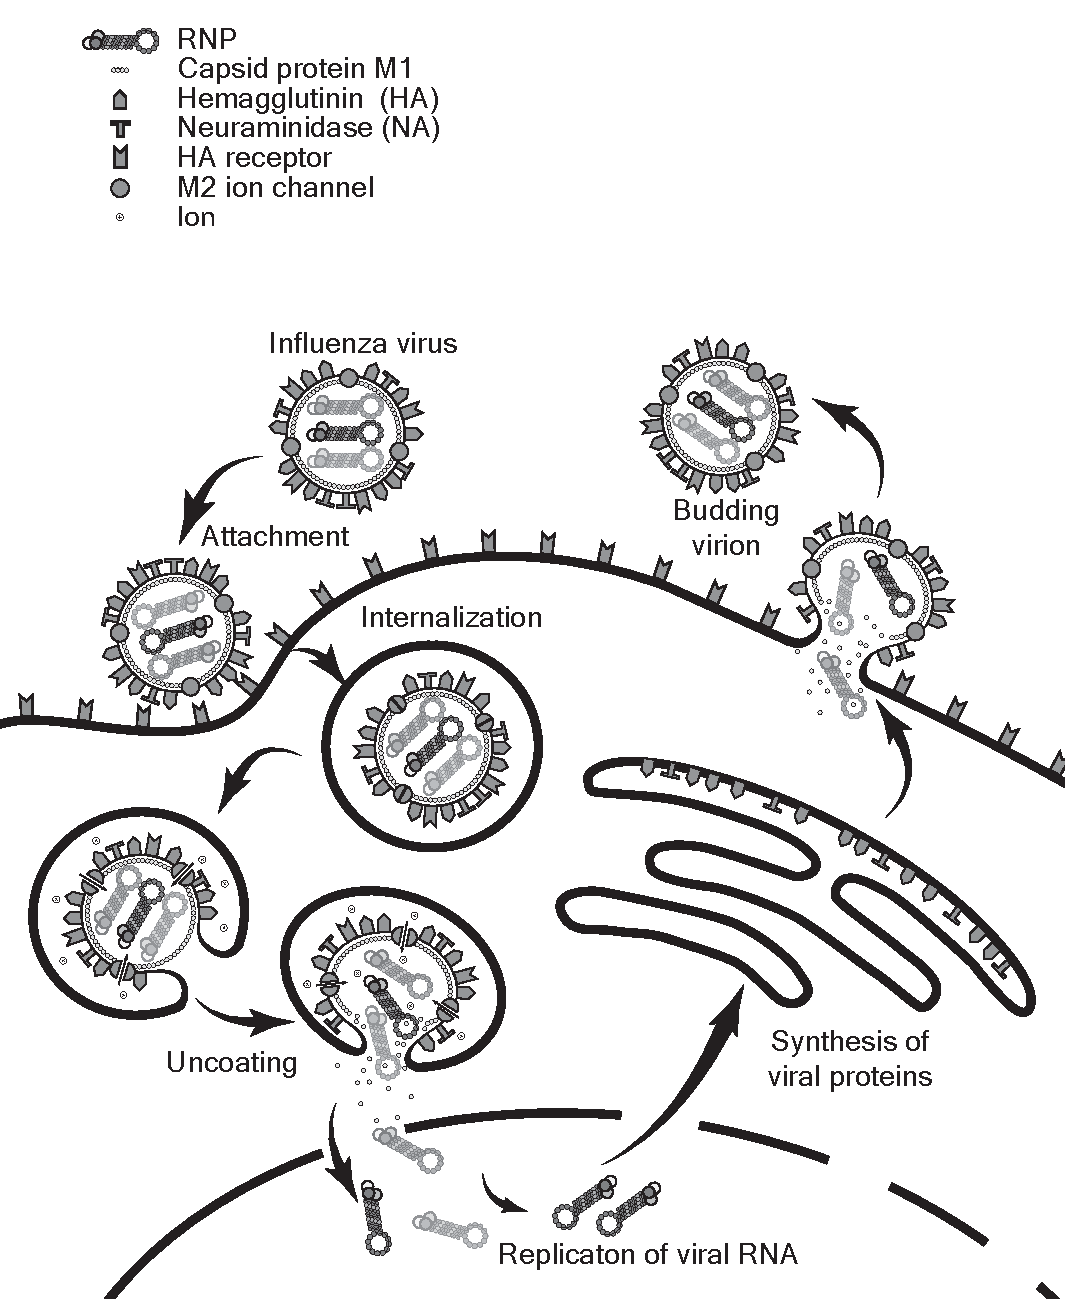
\includegraphics[width=0.95\textwidth, trim={0cm 0cm 0cm 0cm}, clip]{D_chapters/0_introduction/flu_stages.pdf}
\caption[Influenza virus infection course]{Influenza virus infection course. Refer to Figure \ref{figure:fluStructure} for details.}
\label{figure:fluInfectionStages}
\end{center}
\end{figure}